% Esempio per lo stile supsi
\documentclass[twoside]{supsistudent} 
\usepackage{float}
\usepackage{caption}
\usepackage{listings}

% per settare noindent
\setlength{\parindent}{0pt}


% Crea un capitolo senza numerazione che pero` appare nell'indice %
\newcommand{\problemchapter}[1]{%
\chapter*{#1}%
\addcontentsline{toc}{chapter}{#1}%
\markboth{#1}{#1}
}

% Numerazione delle appendici secondo norma
\addto\appendix{
\renewcommand{\thesection}{\Alph{chapter}.\arabic{section}}
\renewcommand{\thesubsection}{\thesection.\arabic{subsection}}}

\setcounter{secnumdepth}{5} 	%per avere più livelli nei titoli
\setcounter{tocdepth}{5}		%per avere più livelli nell'indice


\titolo{Nuovo algoritmo fotogrammetria - Azienda esterna REX SA}
\studente{Terzi Edoardo}
\relatore{Mattei Yari}
\correlatore{-}
\committente{REX SA}
\corso{Ingegneria informatica (TP)}
\modulo{C10051 Progetto di diploma}
\anno{2019}



\begin{document}

\pagenumbering{alph}
\maketitle
\onehalfspacing
\frontmatter

\pagenumbering{roman}
\tableofcontents
% \listoffigures
% \listoftables	

\mainmatter % suddivide in capitolo 1,2,3 ecc.
\pagenumbering{arabic}
\setcounter{page}{1}

\problemchapter{Abstract}
\section{Italiano}
Questo progetto nasce dalla necessità dell'azienda REX di Mendrisio di creare un sistema
per la progettazione di una passerella posta fra i binari di un passo ferroviario. L'azienda
in questine si occupa della produzione, della progettazione e della vendita di molteplici 
articoli tecnici tra i quali le passerelle. 

\bigskip
Inizialmente il sistema, costituito da una piattaforma WEB, si occupava di ricevere in input 
un file DXF realizzato da un geometra dell'azienda. Questo file doveva contenere le rilevazioni 
del geometra, il calcolo delle griglie che costiutiscono la passerella e il disegno di queste. 
Infine la piattaforma generava un documento PDF contenente le istruzioni e il numero di pezzi per 
il montaggio della passerella. Inoltre era possibile gestire i clieniti e gli ordini effettuati 
mediante la piattaforma. 

\bigskip
Attualmente, in seguito a un progetto di semestre svloto da due studenti della SUPSI, la piattaforma 
è migliorata mantenendo sempre l'aspetto relativo alla gestione degli ordini, dei clienti e del PDF 
ma è stato alleggerito il lavoro del geometra. Quest'ultimo ora deve inserire nel file DXF solamente 
le misure effettuate e non deve calcolare a mano le griglie necessarie alla costruzione della passerella.

\bigskip
L'obiettivo di questo progetto di diploma è quello di rendere ancora più semplice ed automatico l'utilizzo 
dell'intero sistema mediante l'utilizzo di tecniche di processamento dell'immagine. In particolare si 
vuole realizzare un algoritmo che sia in grado di rilevare le misure necessarie alla costruzione
delle griglie che compongono la passerella partendo da una o più foto della scena, quindi del passo 
ferroviario dove si vuole fare il lavoro di installazione.

\newpage
\section{Inglese}
This project stems from the need of the REX company in Mendrisio to create a system
for the design of a footbridge between the tracks of a railway pass. The company
in questine it deals with the production, design and sale of multiple
technical articles including the catwalks.

\bigskip
Initially the system, consisting of a WEB platform, took care of receiving input
a DXF file created by a company surveyor. This file had to contain the detections
of the surveyor, the calculation of the grids that make up the gangway and the design of these.
Finally the platform generated a PDF document containing the instructions and the number of pieces per
the assembly of the gangway. It was also possible to manage the customers and the orders placed
via the platform.

\bigskip
Currently, following a semester project carried out by two SUPSI students, the platform
it is improved always maintaining the aspect related to the management of orders, customers and PDF
but the surveyor's work was lightened. The latter must now insert only in the DXF file
the measurements made and must not calculate by hand the necessary grids for the construction of the gangway.

\bigskip
The objective of this diploma project is to make the use even more simple and automatic
of the entire system through the use of image processing techniques. In particular yes
wants to realize an algorithm that is able to detect the measures necessary for the construction
of the grids that make up the walkway starting from one or more photos of the scene, then of the pass
rail where you want to do the installation work.

\newpage
\chapter{Introduzione}
\section{Descrizione}
Rex SA è una società manifatturiera: uno dei molti prodotti commercializzati con il proprio marchio è relativo alla
produzione di passaggi di servizio ferroviari in resina per l’attraversamento nelle stazioni ferroviarie e per uscite di
sicurezza nelle gallerie di treno o metropolitana, articoli commercializzati con il marchio SWISSCROSS GFK.
La sfida del progetto risiede nell’implementazione di un sistema capace di creare e visualizzare in modalità aumentata
(sopra una fotografia) un modello virtuale di un passaggio GFK partendo da un'immagine e attivando automaticamente i
processi di produzione, consegna, installazione e, in seguito, di manutenzione del prodotto.
Grazie alla soluzione proposta, REX sarà in grado rafforzare la propria posizione sul mercato svizzero e modificare il
proprio modello di business per iniziare una vendita di servizi digitali a livello internazionale.
Con il progetto si vuole incrementare la competitività dell’azienda delegando al cliente la progettazione e la visione virtuale
del risultato finale in modalità “self-service” prima ancora di confermare l’ordine tramite la piattaforma cloud,
automatizzando quindi ordinazione, produzione e delivery in un vero e proprio processo di Industria 4.0.

\section{Obiettivi}
L'obiettivo principale è quello di sviluppare un algoritmo in grado di sfruttare le metriche conosciute (scarto binari e modelli
3D di binari, traversine e viterie) per ricavare una matrice omografica tramite la quale calcolare il modello completo di una passerella
sulla base di una immagine. Allineamento e sovrapposizione dei modelli generati da più immagini verranno realizzati sfruttando appositi marcatori
posizionati sul terreno. Sintetizzando l'obiettivo di questo algoritmo è quello di permettere l'estrazione dei punti caratteristici da 
un immagine (features) necessari al calcolo della forma e delle misure di una passerella GFK.

\section{Compiti}
Il compito principale risiede nella creazione quindi di un algoritmo in grado di elaborare un immagine fotografica e ricavarne la relativa matrice omografa.
Tramite questa matrice si potrà "raddrizzare" l'immmagine e quindi calcolare le dimensioni reali del passaggio pedonale
che dovrà quindi essere visualizzato in modalità "realtà aumentata" sopra la fotografia.

\newpage
\chapter{Analisi}
\section{Requisiti}
Descrizione approfondita delle richieste.
\section{Contesto}
Descrizione della scena (costituzione dei binari e terminologia associata). 
\section{Architettura}
\begin{figure}[H]
  \center
  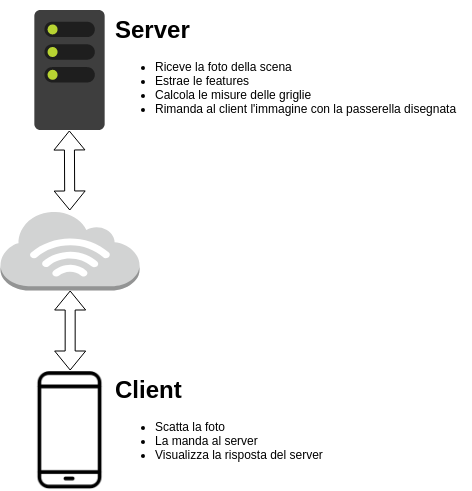
\includegraphics[scale=0.6]{images/Architettura.png}
  \caption{Architettura client-server}
\end{figure}
Descrizione dell'architettura software richiesta.
\chapter{Tecnologie utilizzate}
\section{Hardware}
\subsection{PC per lo sviluppo}
Portatile con Windows 10 Pro 64-bit:
\begin{figure}[H]
  \center
  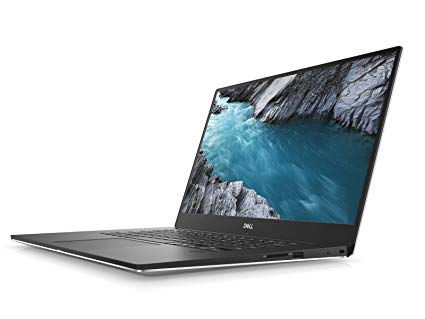
\includegraphics[scale=0.4]{images/pc.jpg}
  \caption{Dell XPS 9570}
\end{figure}
\begin{itemize}
  \item Intel Core i7-8750H CPU 2.20GHz x 12
  \item 16 GB 2 x 8 GB DDR4 a 2.666 MHz
  \item PCIe M.2 2280 da 512 GB
  \item NVIDIA GeForce GTX 1050 Ti con 4 GB di GDDR5
\end{itemize}
\newpage
\subsection{Smartphone per l'acquisizione delle immagini}
Smartphone Android con fotocamera tripla Leica:
\begin{figure}[H]
  \center
  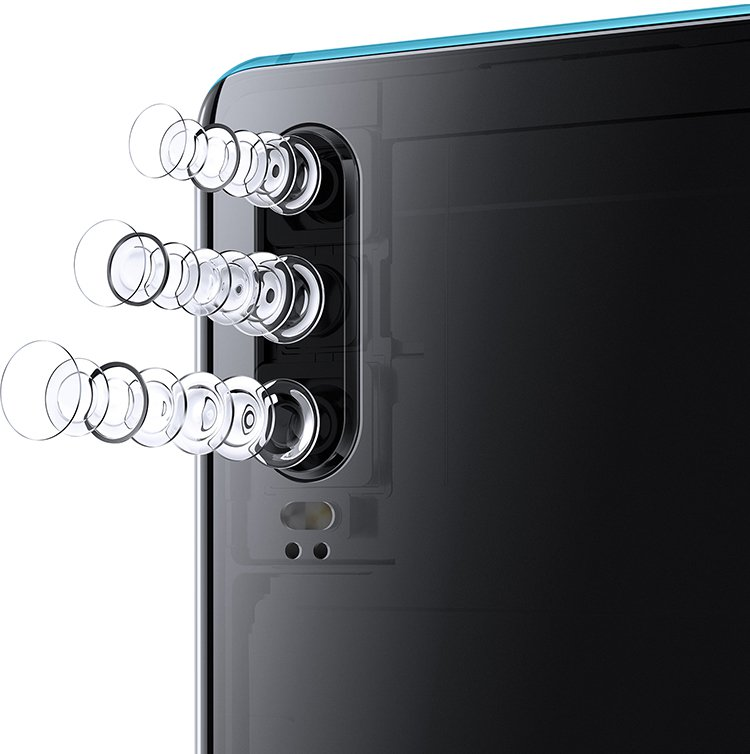
\includegraphics[scale=0.15]{images/smartphone.jpg}
  \caption{Huawei P30}
\end{figure}
\begin{itemize}
  \item 40 MP IMX650 Wide (f/1.8, 27mm, 1/1.7")
  \item 16 MP Ultrawide (f/2.2, 17mm)
  \item 8 MP Telephoto (f/2.4, 80mm, 1/4", OIS)
\end{itemize}
\section{Software}
\subsection{Ambienti di sviluppo, editor}
\noindent
\begin{minipage}[H]{0.49\textwidth} 
  \begin{flushleft}
  IntelliJ IDEA è un ambiente di sviluppo integrato (IDE) per il linguaggio di programmazione Java. 
  Sviluppato da JetBrains (prima conosciuto come IntelliJ), è disponibile sia in licenza Apache che in 
  edizione proprietaria commerciale.
  \end{flushleft}
  \end{minipage}
\hfill
\begin{minipage}[H]{0.49\textwidth}
  \begin{center}
    
\includegraphics[scale=0.1]{images/IdeaLogo.png}
  \end{center}
\end{minipage}

\bigskip
\noindent
\begin{minipage}[H]{0.49\textwidth} 
  \begin{flushleft}
    PyCharm è un ambiente di sviluppo integrato (IDE), in particolare per il linguaggio Python. 
    È sviluppato dalla società ceca JetBrains. Fornisce analisi del codice, un debugger grafico, un tester di unità integrato, 
    integrazione con i sistemi di controllo versione (VCSes) e supporta lo sviluppo Web con Django e Data Science con Anaconda.
    PyCharm è multipiattaforma, con versioni Windows, macOS e Linux. La Community Edition è rilasciata con licenza Apache, c'è anche la Professional Edition con funzionalità extra, 
    rilasciata con licenza proprietaria.
  \end{flushleft}
  \end{minipage}
\hfill
\begin{minipage}[H]{0.49\textwidth}
  \begin{center}
    
\includegraphics[scale=0.1]{images/PyCharm.png}
  \end{center}
\end{minipage}

\bigskip
\noindent
\begin{minipage}[H]{0.49\textwidth} 
  \begin{flushleft}
    Git è un software di controllo versione distribuito utilizzabile da interfaccia a riga di comando, creato da Linus Torvalds nel 2005.
    Git (che nello slang americano significa idiota) nacque per essere un semplice strumento per facilitare lo sviluppo del kernel Linux 
    ed è diventato uno degli strumenti di controllo versione più diffusi. La sua progettazione si ispirò a strumenti (allora proprietari) 
    analoghi come BitKeeper e Monotone.
  \end{flushleft}
  \end{minipage}
\hfill
\begin{minipage}[H]{0.49\textwidth}
  \begin{center}
    
\includegraphics[scale=0.08]{images/git.png}
  \end{center}
\end{minipage}

\bigskip
\noindent
\begin{minipage}[H]{0.49\textwidth} 
  \begin{flushleft}
    Visual Studio Code è un editor di codice sorgente sviluppato da Microsoft per Windows, Linux e macOS. Esso include supporto per debugging, 
    un controllo per Git integrato, Syntax highlighting, IntelliSense, Snippet e refactoring del codice. È un software libero, anche se la versione 
    ufficiale è sotto una licenza proprietaria. Visual Studio Code è basato su Electron, un framework con cui è possibile sviluppare applicazioni Node.js.
  \end{flushleft}
  \end{minipage}
\hfill
\begin{minipage}[H]{0.49\textwidth}
  \begin{center}
    
\includegraphics[scale=0.1]{images/vscode.png}
  \end{center}
\end{minipage}
\subsection{Elaborazione dell'immagine}
\noindent
\begin{minipage}[H]{0.49\textwidth} 
  \begin{flushleft}
    Adobe Photoshop è un software proprietario prodotto dalla Adobe Systems Incorporated specializzato nell'elaborazione di fotografie (fotoritocco) e, più in generale, di immagini digitali.
    Questo programma è in grado di effettuare ritocchi di qualità professionale alle immagini, offrendo enormi possibilità creative grazie ai numerosi filtri e strumenti che permettono di 
    emulare le tecniche utilizzate nei laboratori fotografici per il trattamento delle immagini, le tecniche di pittura e di disegno.
  \end{flushleft}
  \end{minipage}
\hfill
\begin{minipage}[H]{0.49\textwidth}
  \begin{center}
    
\includegraphics[scale=0.1]{images/photoshop.png}
  \end{center}
\end{minipage}

\bigskip
All'interno di questo progetto questo software è stato molto utile al fine di non dover collocarsi fisicamente sulla scena per effettuare una fotografia per ogni approccio tentato. Difatti 
è stato sufficiente apportare le modifiche necessarie alla foto al fine di testare un nuovo approccio. Nei casi in cui un determinato approccio si è rilevato essere valido abbiamo fatto delle 
foto reali della scena per testarlo ulteriormente
\chapter{Diagrammi}
\section{Gantt}
\begin{figure}[H]
  \center
  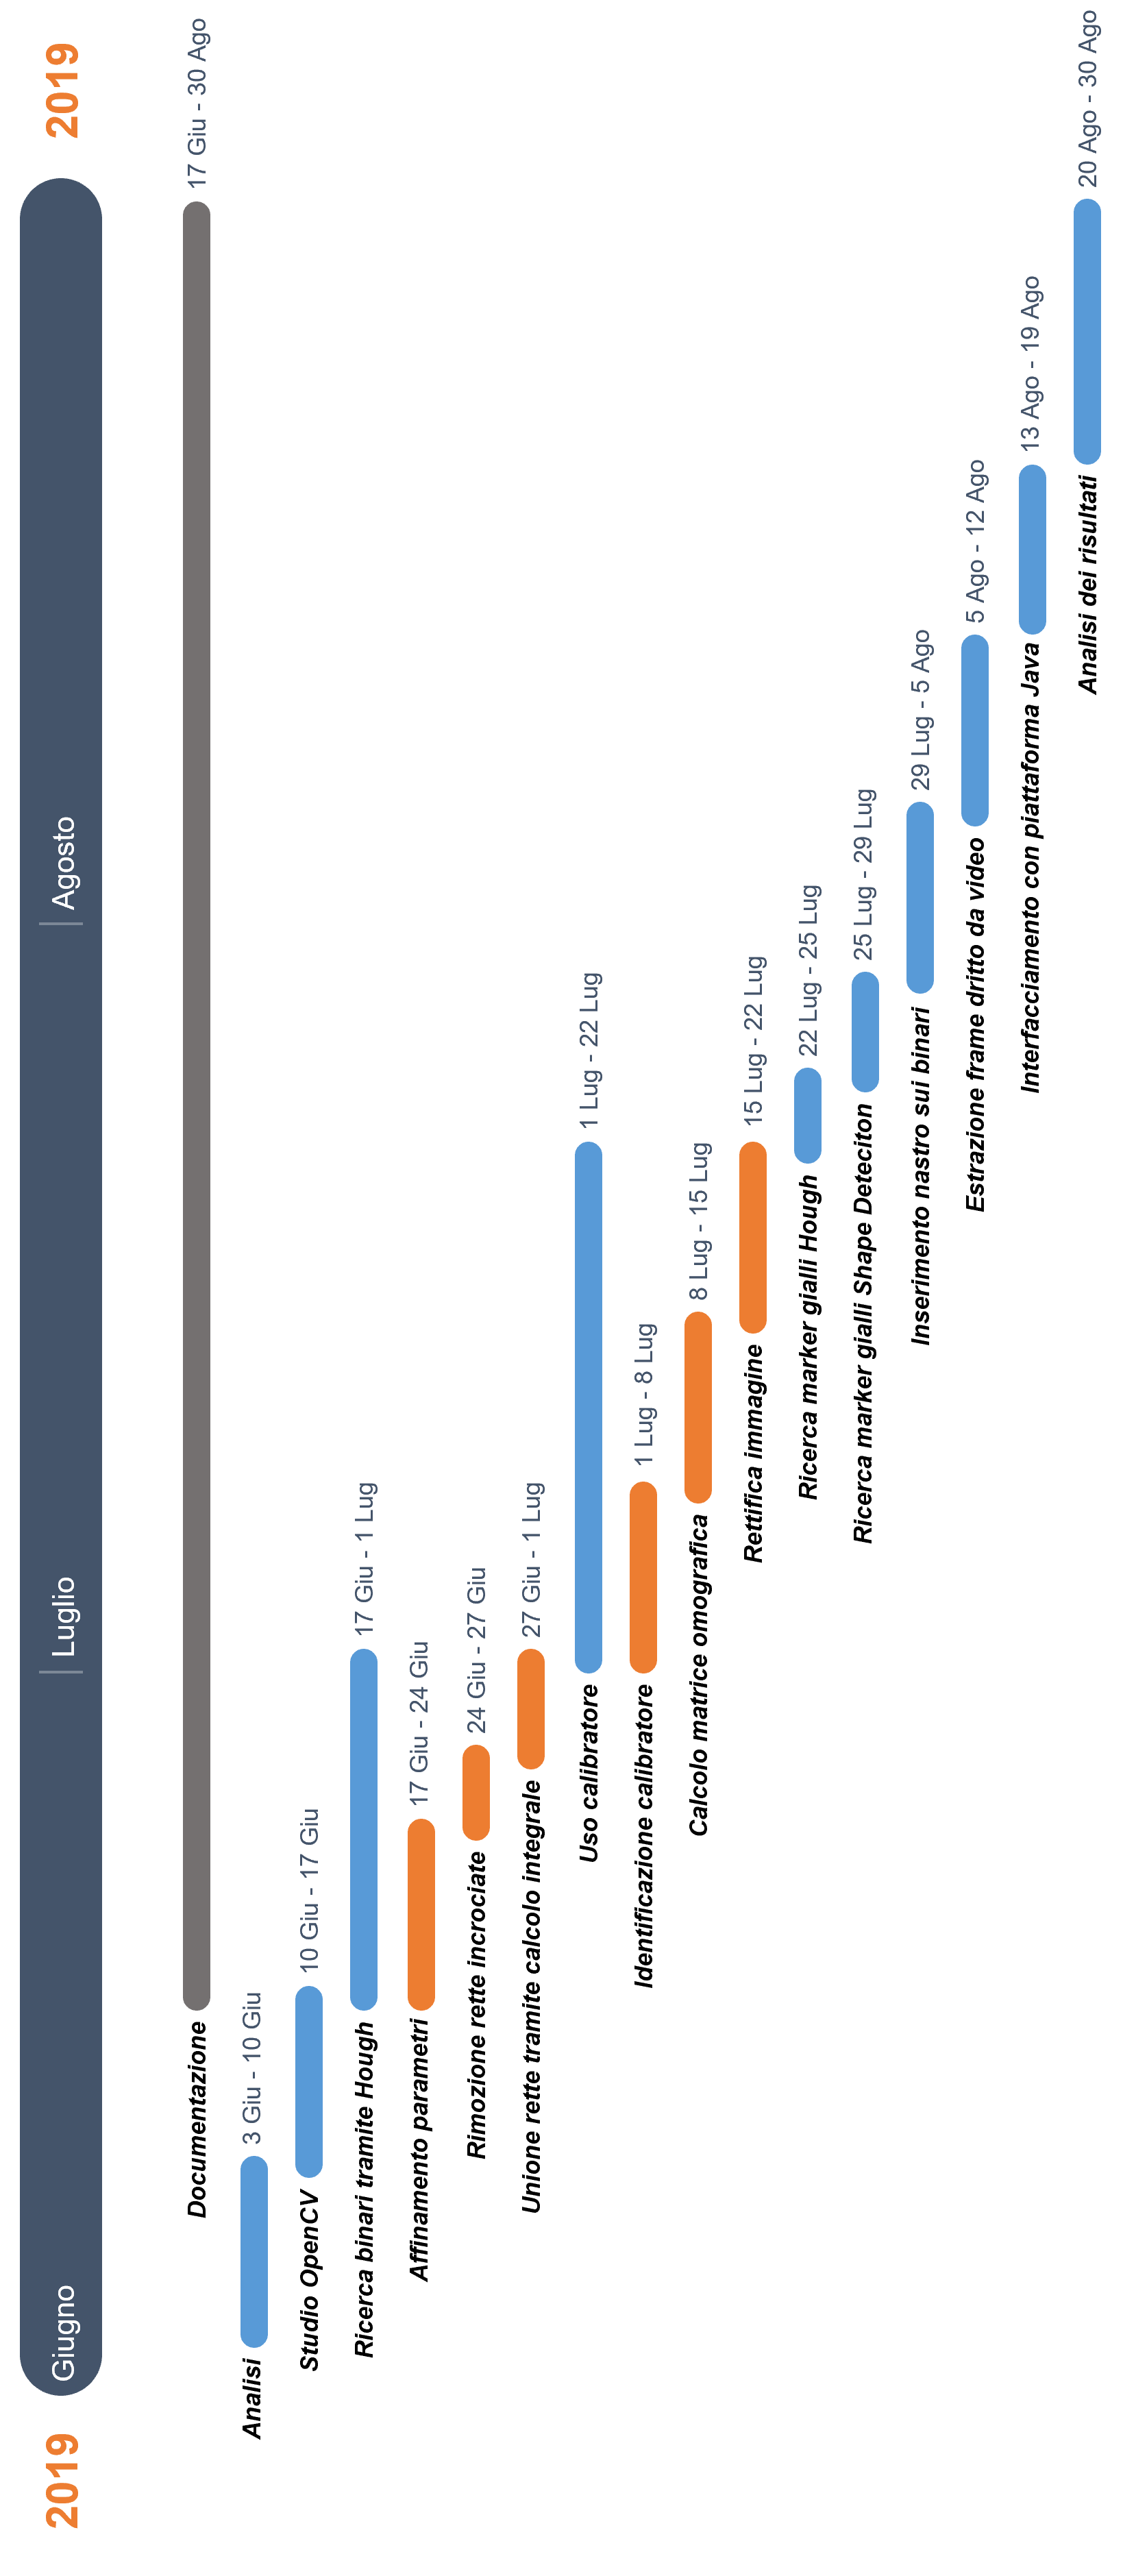
\includegraphics[scale=0.35]{images/Timeline.png}
  \caption{Diagramma}
\end{figure}
Descrizione del diagramma
\section{Casi d'uso}
\begin{figure}[H]
  \center
  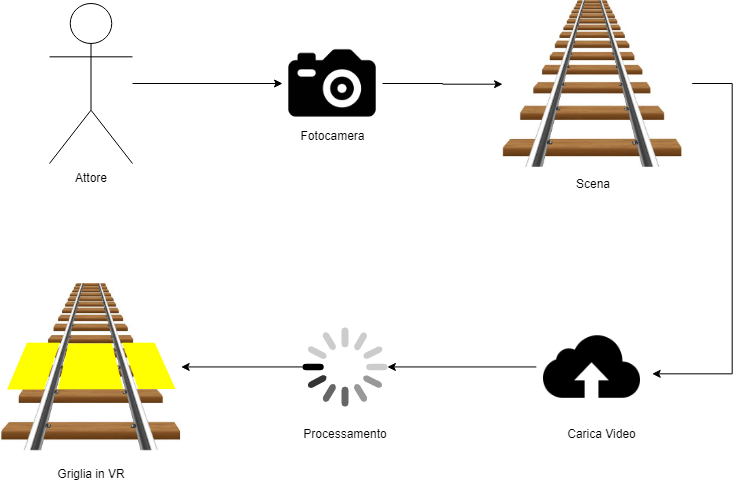
\includegraphics[scale=0.50]{images/UseCase.png}
  \caption{Diagramma}
\end{figure}
Descrizione del diagramma
\section{Sequenza}
\begin{figure}[H]
  \center
  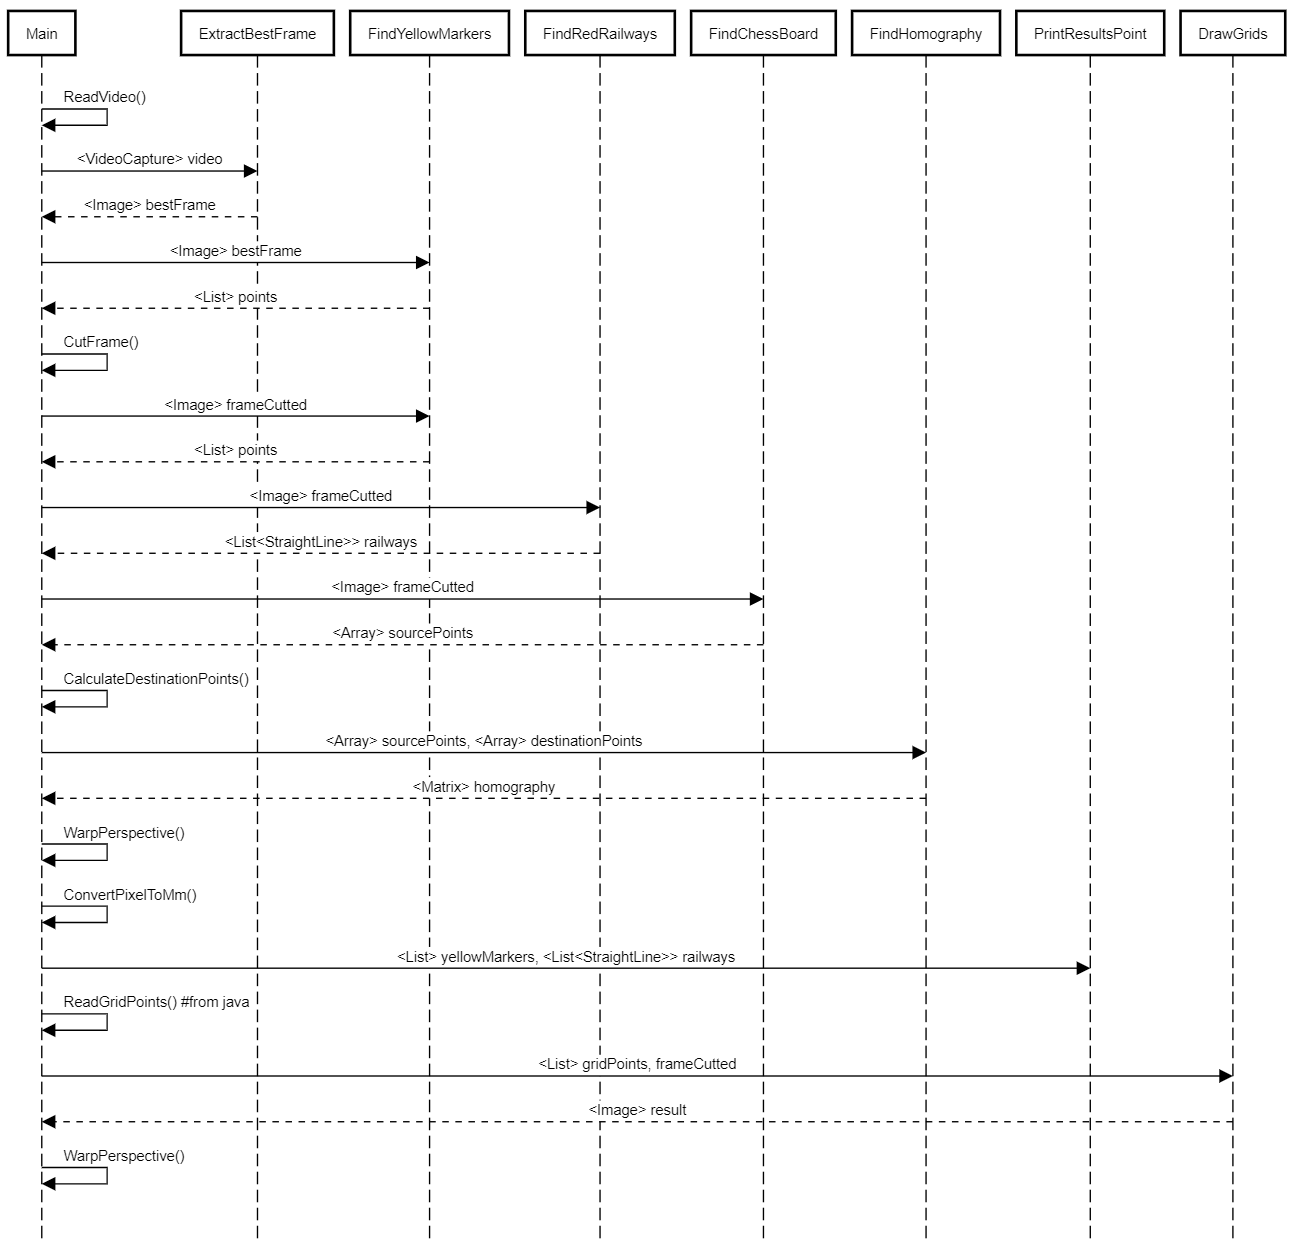
\includegraphics[scale=0.32]{images/Sequence.png}
  \caption{Diagramma}
\end{figure}
Descrizione del diagramma
\chapter{Implementazione}
\section{Linguaggi, librerie, framework}
\subsection{Java}
Java è un linguaggio di programmazione ad alto livello, orientato agli 
oggetti e a tipizzazione statica, che si appoggia sull'omonima piattaforma software, 
specificamente progettato per essere il più possibile indipendente dalla piattaforma 
hardware di esecuzione (tramite compilazione in bytecode prima e interpretazione poi 
da parte di una JVM), sebbene questa caratteristica comporti prestazioni in termini 
di computazione inferiori a quelle di linguaggi direttamente compilati come C e C++ 
ovvero dunque perfettamente adattati alla piattaforma hardware.
Il back-end dell'intera piattaforma è stato sviluppato mediante l'uso di questo linguaggio e 
del framework Spring MVC.
\subsection{Python}
È un linguaggio multi-paradigma che ha tra i principali obiettivi dinamicità, semplicità
e flessibilità. Supporta il paradigma object oriented, la programmazione strutturata e 
molte caratteristiche di programmazione funzionale e riflessione. Le caratteristiche più 
immediatamente riconoscibili di Python sono le variabili non tipizzate e l'uso 
dell'indentazione per la definizione delle specifiche. Altre caratteristiche distintive 
sono l'overloading di operatori e funzioni tramite delegation, la presenza di un 
ricco assortimento di tipi e funzioni di base e librerie standard, sintassi avanzate 
quali slicing e list comprehension.
Abbiamo scelto di utilizzare questo linguaggio in quanto la nota libreria OpenCV, descritta in 
seguito, è completamente supportata e documentata. Difatti gli script in python si occupano 
principalmente del processamento delle immagini. 
\subsection{OpenCV}
OpenCV è una libreria per Computer Vision open source disponibile su http://opencv.org. 
Nel 1999 Gary Bradski, lavorando presso la Intel Corporation, ha lanciato OpenCV con la speranza 
di “migliorare la visione del computer” e l’intelligenza artificiale fornendo una solida 
infrastruttura per tutti coloro che lavorano nel campo dell’image processing. La libreria è 
scritta in C e C++ e funziona su Linux, Windows e Mac OS. Esiste uno sviluppo attivo sulle 
interfacce per Python, Java, MATLAB e altri linguaggi, incluso il porting della libreria su 
Android e iOS per applicazioni mobili. OpenCV ha ricevuto gran parte del suo supporto negli 
anni da Intel e Google, ma soprattutto da Itseez (recentemente acquisita da Intel), che ha 
realizzato la maggior parte dei primi lavori di sviluppo. Infine, la Arraiy Corporation ha aderito per 
mantenere OpenCV.org sempre aperto e gratuito. OpenCV è stata progettata per l'efficienza
computazionale e con una forte attenzione alle applicazioni in tempo reale. È scritta in 
C++, infatti l'uso con questo linguaggio è la soluzione magiormente ottimizzata, inoltre è stata progettata per 
sfruttare a pieno le architetture multi-core. OpenCV utilizza automaticamente la libreria 
IPP appropriata (designata all’ottimizzazione multi-core) in fase di esecuzione se tale 
libreria è installata. A partire da OpenCV 3.0, Intel ha concesso al team OpenCV e alla 
comunità OpenCV un sottoinsieme gratuito di IPP (soprannominato IPPICV), che è integrato e 
accelera OpenCV per impostazione predefinita. Uno degli obiettivi di OpenCV è fornire 
un'infrastruttura di Computer Vision di facile utilizzo al fine di aiutare gli utilizzatori 
a creare rapidamente applicazioni abbastanza sofisticate. La libreria contiene 
oltre 500 funzioni che coprono molte aree della Computer Vision, compreso imaging medico, 
sicurezza, interfaccia utente, calibrazione della fotocamera, visione stereo e robotica. 
Questo perché la visione artificiale e l'apprendimento automatico spesso vanno “mano nella 
mano”, OpenCV contiene anche una libreria di Machine Learning completa e generica (modulo ML). 
Questa “sotto libreria” è focalizzata sul riconoscimento di modelli statistici e clustering. 
Il modulo ML è estremamente utile per i compiti di Computer Vision che sono al centro della missione 
di OpenCV, ma è abbastanza generale da essere utilizzata per qualsiasi problema di 
apprendimento automatico.
\section{Feature detection}
In computer vision, e nell'elaborazione digitale delle immagini, il concetto di rilevamento
di caratteristiche (feature detection) o riconoscimento di caratteristiche racchiude una 
serie di metodi per l'estrapolazione di informazioni da una immagine e per prendere 
decisioni locali sull'esistenza o meno di una caratteristica in quel determinato punto. 
Le caratteristiche risultanti saranno un sottoinsieme del dominio dell'immagine, spesso 
in forma di punti isolati, curve continue o regioni connesse.
Non esiste una definizione universale ed esatta di cosa costituisca una caratteristica 
dell'immagine (image feature), e la definizione esatta spesso dipende dal problema o dal 
tipo di applicazione. Le caratteristiche sono usate spesso come punto di partenza da molti 
algoritmi di computer vision.
Una proprietà desiderabile per un rilevatore di caratteristiche è la ripetibilità: 
la stessa caratteristica dovrebbe essere rilevata in due o più differenti immagini della stessa scena.
È un'operazione di elaborazione delle immagini di basso livello, che ed esamina ogni pixel. 
È la prima operazione che si fa su un'immagine. Se invece fa parte di un algoritmo, 
allora di solito esamina solamente la regione individuata.
\subsection{Primo Approccio}
\subsubsection{Trasformata di Hough}
In computer vision esistono innumerevoli tecniche per l'estrazione delle features. Una 
di queste è la trasformata di Hough, utilizzata per individuare linee all'interno di una 
immagine. Ideata nella sua forma base agli inizi degli anni '60 da Paul Hough, fu in 
seguito perfezionata in una forma generalizzata e resa popolare nel 1981 da Dana H. 
Ballard, docente di informatica dell'università del Texas.
La trasformata di Hough necessita di un passo di preprocessing finalizzato all'Edge 
Detection (es Canny Edge Detection). L'immagine così ottenuta sarà una immagine in bianco e nero
dove i pixel bianchi rappresentano gli Edge, ovvero i contorni dei soggetti 
rappresentati. L'obiettivo della trasformata di Hough è di identificare quali di questi 
contorni rappresentino una linea retta: se più pixel di Edge sono allineati, anche se non 
connessi tra loro, viene individuata una linea nell'immagine.
Per rappresentare una linea retta servono due parametri: un coefficiente angolare $m$ e 
una ordinata all'origine $c$. Considerato un singolo punto, questo appartiene a infinite 
rette della forma $y=mx+c$, al variare di $m$ e $c$. Dobbiamo quindi stabilire quali coppie 
$(m,c)$ siano in grado di individuare al meglio gli allineamenti di pixel.
L'idea della trasformata di Hough è di rappresentare le rette nello spazio parametrico 
$m-c$. In questo modo preso un punto $(x,y)$ l'equazione $y=mx+c$ andrà a rappresentare 
una sola retta invece di infinite. Nello spazio parametrico vengono quindi rappresentate 
tante rette quanti sono i pixel di edge. Se queste rette si intersecano, i due punti 
corrispondenti dell'immagine risulteranno allineati sulla retta con i coefficienti 
$(m,c)$ corrispondenti. La tecnica sembra quindi funzionare: le rette corrispondenti ad 
un alto numero di intersezioni nello spazio parametrico sono le linee che volevamo 
ottenere.
\begin{figure}[H]
  \center
  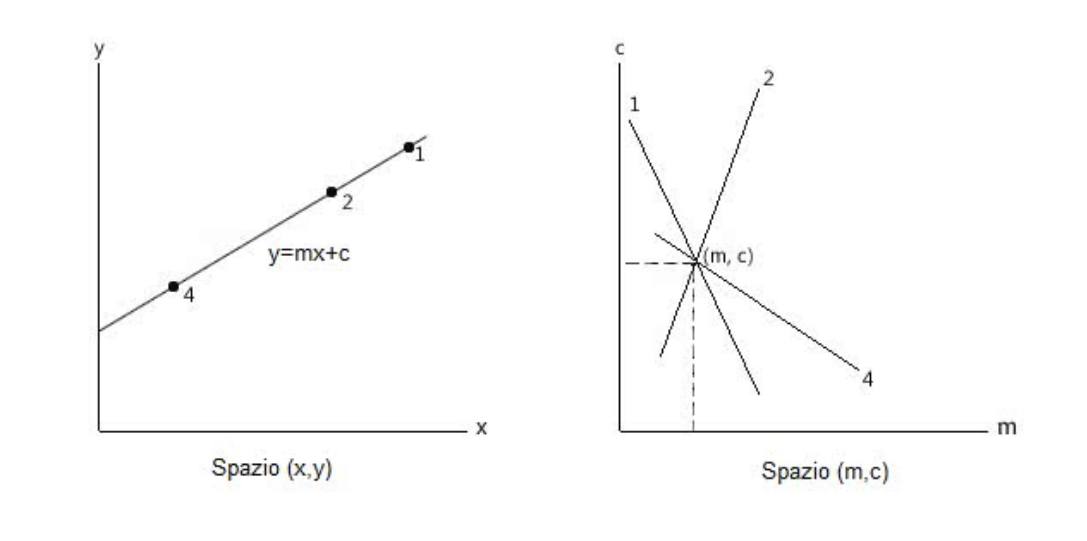
\includegraphics[scale=0.38]{images/spazioMC.png}
  \caption{I parametri m e q vengono mappati nello spazio parametrico e la linea è 
  individuata dall'intersezione delle rette.}
\end{figure}

La trasformata però in questa forma presenta dei problemi che non la rendono applicabile 
su un calcolatore. Infatti per linee verticali il coefficiente angolare $m$ tende all'infinito, 
contrastando le limitazioni di memoria di ogni computer. Si ricorre quindi ad una versione 
detta forma normale dove le rette vengono rappresentate mediante la forma $xcos\theta+ysin\theta=r$.
I parametri $\theta$ e $r$ sono rispettivamente l'angolo e la distanza della retta dall'origine. 
Quantizzando $\theta$ e utilizzando come spazio parametrico $\theta-r$ si risolve quindi il problema 
della finitezza della memoria.
All'interno della libreria OpenCV la traformata di Hough si ottiene tramite la funzione:
\begin{lstlisting}[language=Python]
def HoughLinesP(image, rho, theta, threshold, lines=None, 
                minLineLength=None, maxLineGap=None):
\end{lstlisting}
\begin{itemize}
  \item \textbf{image:} puntatore all'immagine degli edge ottenuta tramite un algoritmo di 
  Edge Detection.
  \item \textbf{rho:} spessore in pixel delle linee rappresentate nello spazio parametrico. 
  Viene utilizzato per accorpare tra loro intersezioni vicine.
  \item \textbf{threshold:} soglia sul numero di intersezioni che si devono ottenere 
  affinchè una linea sia identificata come tale.
  \item \textbf{lines:} struttura dove la funzione scrive le linee, tipicamente sotto forma 
  di CvMemoryStorage.
  \item \textbf{minLineLength:} rappresenta la lunghezza minima di una linea.
  \item \textbf{maxLineGap:} rappresenta a distanza tra punti sulla stessa retta, per 
  spezzarla in due linee differenti.
\end{itemize}
\subsubsection{Binari}
\begin{figure}[H]
  \center
  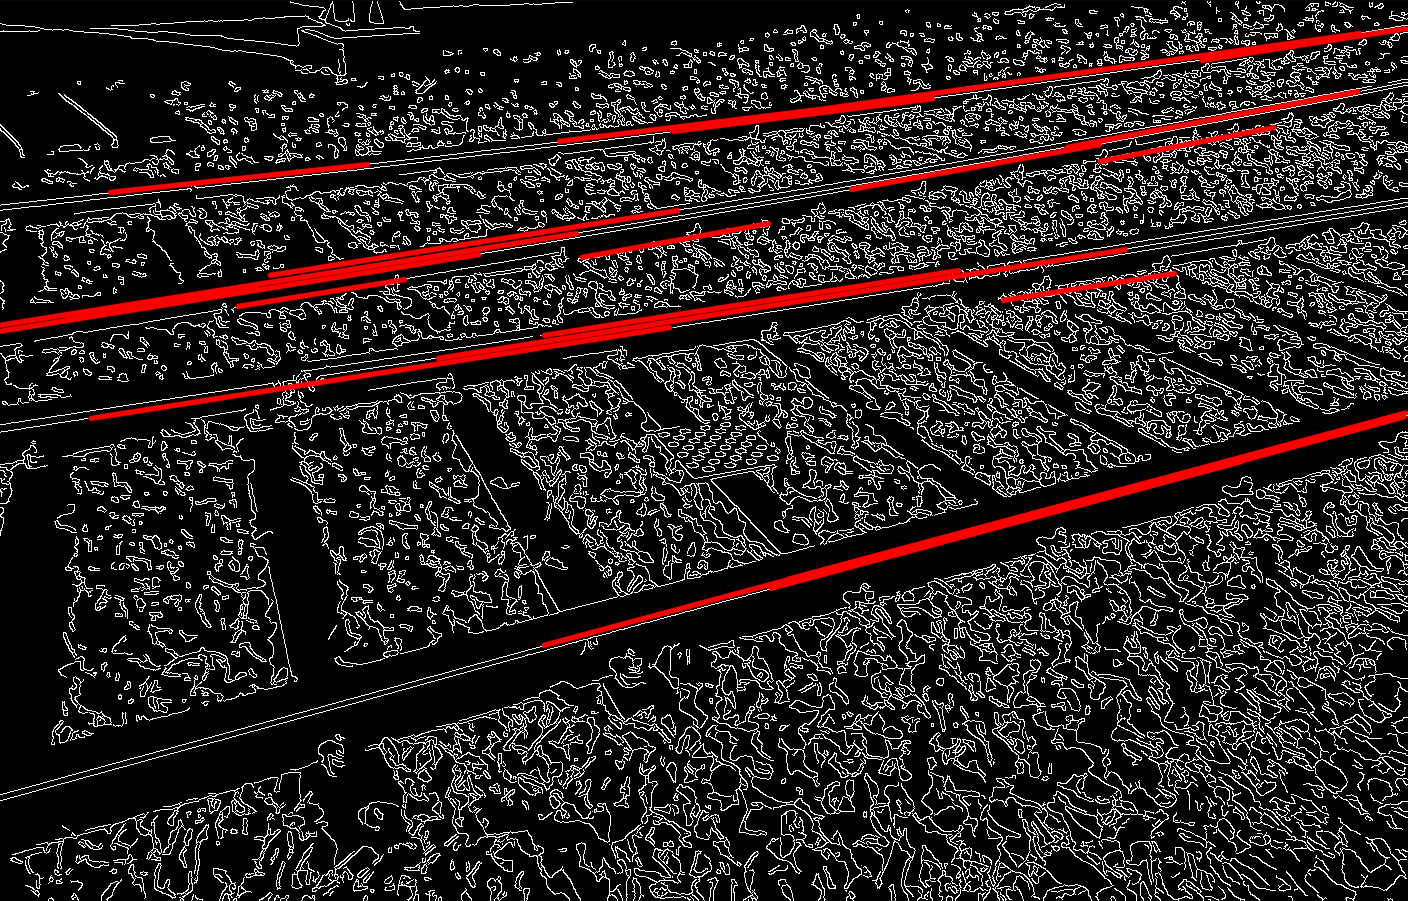
\includegraphics[scale=0.25]{images/houghLines.png}
  \caption{Ricerca dei binari mediante la trasformata di Hough}
\end{figure}
Come si evince dall'immagine sopra, mediante la trasformata di Hough è possibile identificare 
i binari all'interno di una foto. Al fine di identificare solo i binari e non altre linee rette
è necessario settare correttamente i parametri, in particolar modo il valore di threshold e 
la lunghezza minima delle rette. Per torvare il valore ottimale di threshold abbiamo usato la soglia OTSU 
calcolata sfruttanto la varianza tra classi di pixel (l'algoritmo che calcola questa soglia è implementato nativamente
nella libreria OpenCV). Invece per determinare la lunghezza minima delle linee abbiamo effettuato un calcolo 
assumendo che un binario sia lungo quanto la larghezza o lunghezza della foto. Tuttavia, si può notare
come un binario può essere identificato da più rette. Inoltre, nonostante il settaggio corretto dei parametri 
è comunque possibile che vengano rilevate linee che non centrano nulla con i binari. L'approccio scelto
per risolvere questi due problemi è di tipo matematico. Per identificare un binario con una sola abbiamo deciso di raggupparle
sfruttando l'area sottesa alla retta trovata, ovvero l'integrale, assumendo che due rette che rappresentano lo stesso binario 
hanno un'area circa uguale. Infine per identificare solo i binari e non altre linee rette abbiamo rimosso 
tutte le rette che si intersecano all'interno dello spazio definito dalla foto e per maggiore sicurezza l'immagine è anche stata 
sfocata mediante un filtro gaussiano al fine di far rimanere in evidenza solo le linee dei binari.
\begin{figure}[H]
  \center
  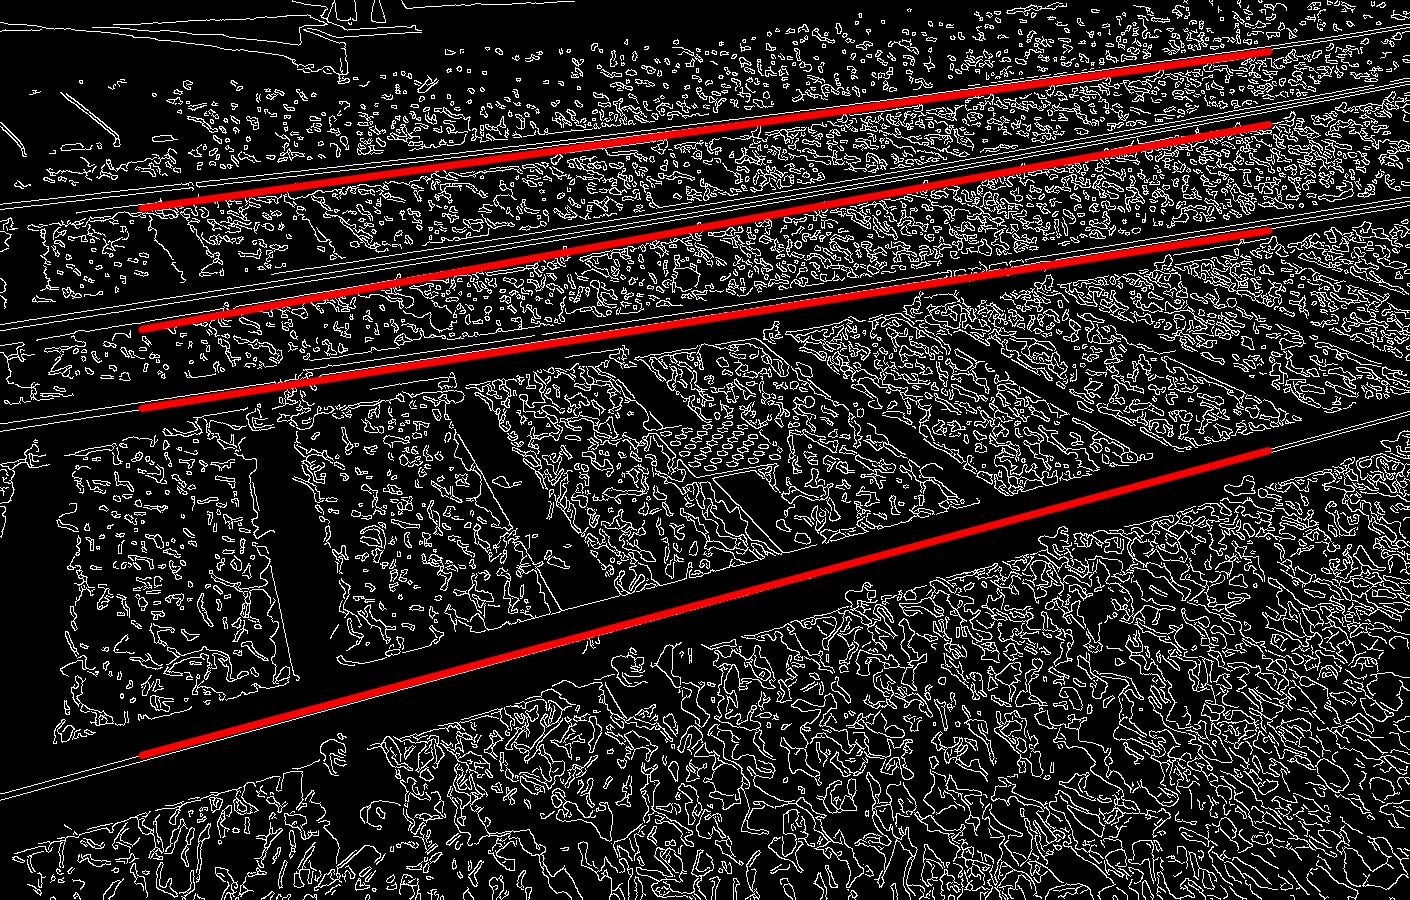
\includegraphics[scale=0.25]{images/houghLinesMerged.jpg}
  \caption{Risultato filtraggi matematici}
\end{figure}
Il risultato ottenuto sembra promettere bene tuttavia, sfruttando questa tecnica si rischia di non fare distinzione tra 
il lato interno o esterno del binario. Inoltre non è possibile determinare se la linea identifica il binari sullo stesso piano. 
Come soluzione abbiamo deciso di sfruttare i bulloni delle traversine messe in risalto con del nastro rosso. Posizionandone anche solo 
quattro è possibile identificare correttamente i binari. 
\subsubsection{Punti}
\begin{figure}[H]
  \center
  
\includegraphics[scale=0.40]{images/empty.jpg}
  \caption{Rilevamento delle palline da tennis}
\end{figure}
Per rilevare in modo accurato le palline da tennis che vanno a definire la passerella abbiamo dapprima effettuato un 
filtraggio sul colore giallo come segue:
\begin{figure}[H]
  \center
  
\includegraphics[scale=0.40]{images/empty.jpg}
  \caption{Filtraggio sul colore delle palline}
\end{figure}
Nell'immagine sopra sono rimaste solo le palline il resto è stato settato a 0 (quindi nero), in questo modo ci è stato possibile ricercare i contorni delle regioni di colore giallo e 
identificare così i 4 punti. Per fare questo abbiamo risfruttato l'algoritmo di Hough mediante la seguente funzione:
\begin{lstlisting}[language=Python]
def HoughCircles(image, method, dp, minDist, circles=None, 
                 param1=None, param2=None, minRadius=None, 
                 maxRadius=None):
\end{lstlisting}
\begin{itemize}
  \item \textbf{image:} puntatore all'immagine degli edge ottenuta tramite un algoritmo di 
  Edge Detection.
  \item \textbf{method:} metodo sfruttato per il rilevamento di circonferenze, 
  l'unico attualmnete disponibile e quello del gradiente.
  \item \textbf{dp:} rapporto inverso della risoluzione (default 1).
  \item \textbf{minDist:} distanza minima tra il centro delle circonferenze rilevate.
  \item \textbf{circles:} array di output.
  \item \textbf{param1:} soglia superiore per il processo di edge detection (Canny).
  \item \textbf{param2:} soglia per il rilevamento del centro, più è bassa più si 
  rischiano falsi positivi.
  \item \textbf{minRadius:} raggio minimo delle circonferenze da rilevare.
  \item \textbf{maxRadius:} raggio massimo delle circonferenze da rilevare.
\end{itemize}
\subsection{Secondo approccio}
\subsubsection{Shape detection}
Questo apporccio abbandona comoletamente l'uso di Hough per il rilevamento di linne e circonferenze ma comunque sfrutta il filtraggio del colore
al fine di escludere oggetti e fomre irrilevanti. Una volta effettuato questo filtraggio nell'immagine ottenuta viene fatta una pulizia del 
rumore effettuando un erosione seguita da una dilatiazione. Così facendo vengono rimossi quei punti troppo piccoli per essere classificati come features.
Successiveamente viene fatta una detezione dei controni sfuttando il metodo messo a disposizione della libreria OpenCV \textit{findContours()}. Infine i contorni delle 
shape aree non nere (shapes) vengono ordinati in base alla dimensione dell'area che delimitano (dalla shape più grande a quella più piccola). Infine vengono prese in 
considerazione solo il numero di shape che si vuole ricercare. Nel caso delle palline da tesnnis 4 mentre nel caso dei binari 2. 
\subsubsection{Binari}
Non potendo definire un range di colori che isolasse in modo appropriato i binari abbiamo deciso di applicare del nastro isolante di fianco ai bulloni
che tengono insieme binari e traviersine: 
\begin{figure}[H]
  \center
  
\includegraphics[scale=0.40]{images/empty.jpg}
  \caption{Nastro rosso opportunamente applicato sulla scena}
\end{figure}
Una volta effettuato il classico filtragigo sul colore sono state rilevate le shapes che definiscono i pezzi di nastro, 
Successivamente sono state tracciate delle linee rette sopra il bordo più esterno della shape rilevata. In questo modo siamo 
riusciti, grazie al rapporto millimetri-pixel (calcolato in seguito) a determinare la posizione dei binari. 
\begin{figure}[H]
  \center
  
\includegraphics[scale=0.40]{images/empty.jpg}
  \caption{Linea retta che identifica il binario}
\end{figure}
\subsubsection{Punti}
Come per i binari abbiamo effettuato un filtragigo sul colore, giallo in questo caso, e abbiamo identificato con buona precisone 
le aree che delimitano le palline. Successivamente, per ridurre al minimo l'errore è stato scelto il punto più basso di quest'area. 
\begin{figure}[H]
  \center
  
\includegraphics[scale=0.40]{images/empty.jpg}
  \caption{Risultato}
\end{figure}
\subsection{Foto o video}
Inizialmente abbiamo sfruttato solo una foto della scena per effettuare tutti i rilevamenti del caso. Tuttavia, procedendo con lo sviluppo dell'algoritmo, 
ci siamo accorti che se il calibratore non era perfettamente allineato orizzontalmente e veritcalmente si otteneva un'immagine raddrizzata piena di errori di distorsione. 
Essendo quasi impossibile fare uno scatto preciso abbiamo deciso di fare un video della scena. Ogni frame del video viene analizzato e ne viene estratto quello 
migliore basandosi sulla posizione e inclinazione del calibratore. 
\subsection{Approccio scelto}
Dopo numerosi tentativi abbiamo scelto di sfruttare la combinazione della shape detection in combinazione con un video della scena. In questo modo non si sono presentati ne 
i problemi relativi alla distorsione dell'immagine in fase di rettifica (raddrizzamento dell'immagine con visione dall'alto) ne tutti i problemi derivanti dall'uso dell'algoritmo di Hough.
In particolare quest'ultimo richiede una serie di parametri specifici che possono variare in funzione dell'illuminazione della scena o della distanza a cui si pone l'utente. Va detto che, utilizzando
questo approccio non si sono eliminati definitavamente questo genere di problmeatiche, tuttavia si sono ridotte notevolmente.
\section{Calibratore}
\begin{figure}[H]
  \center
  
\includegraphics[scale=0.5]{images/empty.jpg}
  \caption{Foto dei binari co il calibratore poggiato sulle traversine}
\end{figure}
Come si evince dall'immagine abbiamo deciso di collocare un calibratore, ovvero una scacchiera $5 x 8$, sulla scena. 
Questo calibratore è stato realizzato stampando su due fogli A3 la scacchiera in questione. Ne sono note tutte le misure con 
precisione al millimetro. Mediante il seguente metodo, presente all'interno della libreria OpenCV siamo riusciti ad indentificarne con
accuratezza i vertici. 
\begin{lstlisting}[language=Python]
  def findChessboardCorners(image, patternSize, corners=None,
   flags=None):
\end{lstlisting}
\begin{itemize}
  \item \textbf{image:} puntatore all'immagine in scala di grigi contenente il calibratore
  \item \textbf{patternSize:} dimensioni (righe per colonne) del calibratore, si intendono i vertici quindi occorre togliere 1 ad entrambi i valori.
  \item \textbf{corners:} vettore di output.
  \item \textbf{flags:} eventuali flags aggiuntivi per specificare il metodo con cui viene rilevato il calibratore, di default 0.
\end{itemize}
Il risultato ottenuto è il seguente:
\begin{figure}[H]
  \center
  
\includegraphics[scale=0.5]{images/empty.jpg}
  \caption{Risultato della detezione evidenzato dal metodo drawChessboard()}
\end{figure}
Una volta rilevato il calibratore abbiamo ricondotto i suoi vertici (sourcePoints), che nell'immagine formano un trapezio a causa dell'effetto prospettico, ad un rettangolo come nella realtà (destinationPoints). 
Così facendo abbiamo sfruttato i punti per calcolare la matrice omografica (descritta in seguito) la quale ci ha permesso di raddrizzare l'immagine 
avendo una visione dall'allto della scena. 
\begin{figure}[H]
  \center
  
\includegraphics[scale=0.5]{images/empty.jpg}
  \caption{Prima e dopo l'applicazione della matrice}
\end{figure}
Per applicare la matrice all'immagine abbiamo utilizzato un altro metodo della libreria OpenCV: 
\begin{lstlisting}[language=Python]
  def warpPerspective(src, M, dsize, dst=None, flags=None,
   borderMode=None, borderValue=None):
\end{lstlisting}
\begin{itemize}
  \item \textbf{src:} puntatore all'immagine orriginale.
  \item \textbf{M:} Matrice omografica.
  \item \textbf{dsize:} dimensioni dell'immagine di destinazione.
  \item \textbf{dst:} matrice di output.
  \item \textbf{flags:} Metodo di interpolazione dei pixel da usare.
  \item \textbf{borderMode:} Metodo di estrapolazione dei pixel. 
\end{itemize}
Tuttavia, prima di applicare la matrice all'intera immagine si è reso necessario applicarla solo ai vertici dell'immagine di partenza in quanto la 
trasformazione omografica distorce e dilata l'immagine alternadone le dimensioni, sapendo che valore assumono i vertici dell'immagine di partenza abbiamo
calcolato le dimensioni dell'immagine di destinazione. Sfruttando questa tecnica non ci sono state perdite di informazione (in questo caso tagli nell'immagine).
\section{Matrice Omografica}
In matematica e geometria una omografia è una relazione tra punti di due spazi tali per cui ogni punto di uno spazio corrisponde ad uno ed un solo
punto del secondo spazio. In Computer Vison il concetto alla base è circa lo stesso: definiamo l'omografia planare come una “mappatura proiettiva” da
una superficie per un’altra. L’esempio più classico di omografia, che viene usato da ognuno di noi quotidianamente, è sicuramente la mappatura dei
punti su una superficie planare bidimensionale fatta dal sensore della nostra macchina fotografica. È possibile esprimere questa mappatura come
moltiplicazione di matrici. Sfruttando le coordinate omogenee definiamo un punto nella realtà $\vec{Q}$ e la sua “mappatura” $\vec{q}$ effettuata dal sensore:
\[
\vec{Q} = \Spvek[c]{X;Y;Z;1}\quad e \quad \vec{q} = \Spvek[c]{x;y;1}
\]
allora possiamo esprimere l'azione dell'omografia semplicemente come:
\[\vec{q} = s \cdot H \cdot \vec{Q}\]
Nella formula appena vista abbiamo introdotto il parametro $s$, quest’ultimo è un fattore di scala arbitrario convenzionalmente separato da $H$. L'osservazione 
più importante è che $H$ è composta da due parti: la trasformazione fisica, che localizza essenzialmente il piano dell'oggetto che stiamo visualizzando e la 
proiezione, che introduce la matrice intrinseca della fotocamera.
\begin{figure}[H]
  \center
  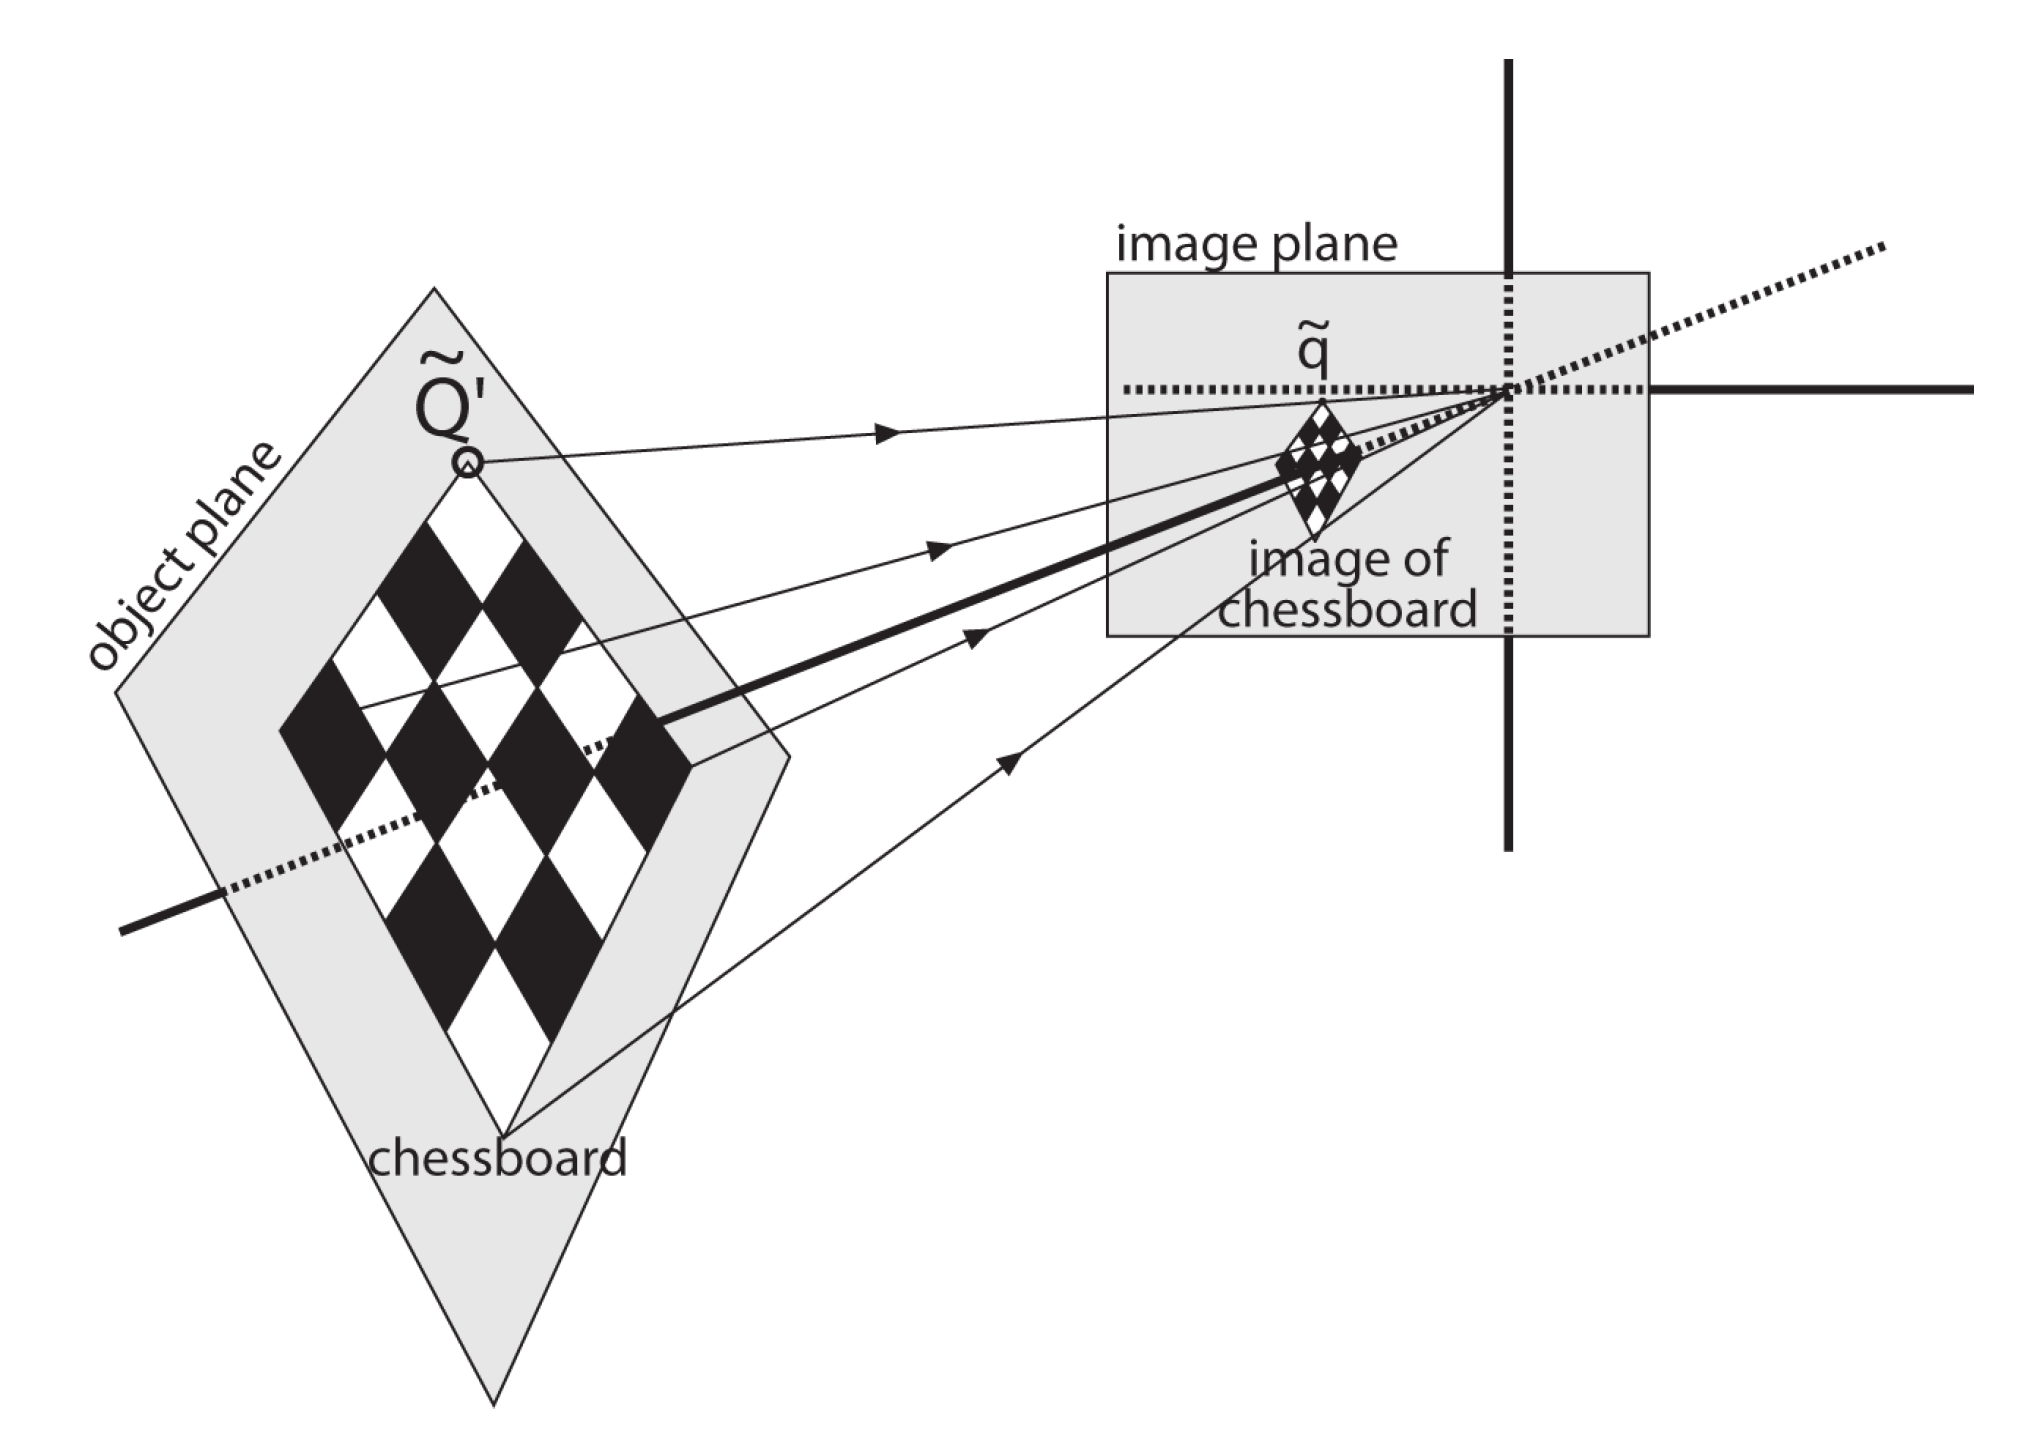
\includegraphics[scale=0.50]{images/Omografia.png}
  \caption{Vista di un oggetto planare come descritto dall'omografia: una mappatura 
  (dal piano dell'oggetto al piano dell'immagine) che comprende contemporaneamente le 
  relative posizioni di questi due piani e matrice di proiezione della telecamera.}
\end{figure}
La parte di trasformazione fisica è la somma degli effetti di alcune rotazioni $R$ e alcune traslazioni $\vec{t}$ che mettono in relazione il piano che stiamo 
visualizzando con il piano dell'immagine. Considerando che stiamo lavorando in coordinate omogenee, possiamo combinare queste trasformazioni in una 
sola matrice come segue:
\[W = [\quad R \quad \vec{t} \quad ]\]
Quindi, l'azione della matrice della fotocamera $M$, che già sappiamo esprimere in coordinate proiettive, viene moltiplicata per $\vec{Q}$, che produce:
\[\vec{q} = s \cdot M \cdot W \cdot \vec{Q}\]
Dove:
\[  
  M = \begin{bmatrix}
    f_{x} & 0 & c_{x}  \\
    0 & f_{x} & c_{y}  \\
    0 & 0 & 1  \\
  \end{bmatrix}
\]
Tuttavia, considerando che non ci interessa una coordinata $\vec{Q}$ definita su tutto lo spazio ma una coordinata $\vec{Q'}$ definita solo sul piano che stiamo guardando. 
Ciò consente una leggera semplificazione. Senza perdita di generalità, possiamo scegliere di definire il piano dell'oggetto in modo che $Z = 0$. Possiamo farlo 
perché, se suddividiamo anche la matrice di rotazione in tre colonne $3 x 1$ (ad es. $R = [\quad \vec{r_{1}} \quad \vec{r_{2}} \quad \vec{r_{3}} \quad ]$), una di quelle colonne non è più necessaria. In particolare:
\[
  \Spvek[c]{x;y;1} = 
  s \cdot M \cdot \begin{bmatrix} \quad \vec{r_{1}} \quad \vec{r_{2}} \quad \vec{r_{3}} \quad \vec{t} \quad \quad \end{bmatrix} \cdot \Spvek[c]{X;Y;0;1} = 
  s \cdot M \cdot \begin{bmatrix} \quad \vec{r_{1}} \quad \vec{r_{2}} \quad \vec{t} \quad \quad \end{bmatrix} \cdot \Spvek[c]{X;Y;1}
\]
La matrice di omografia $H$ che mappa i punti di un oggetto planare sul sensore è quindi descritta completamente da $H = s \cdot M \cdot [\quad \vec{r_{1}} \quad \vec{r_{2}} \quad \vec{t} \quad ]$, dove:
\[\vec{q} = s \cdot H \cdot \vec{Q'}\]
Possiamo osservare che $H$ ora è una matrice $3 x 3$. OpenCV utilizza le equazioni precedenti per calcolare la matrice di omografica. Utilizza più immagini dello stesso oggetto per calcolare sia le singole 
traslazioni e rotazioni per ciascuna vista nonché i valori intrinseci (che sono gli stessi per tutte le viste). Come abbiamo discusso, la rotazione è 
descritta da tre angoli e la traslazione è definita da tre offset; quindi ci sono sei incognite per ogni vista. Questo va bene, perché un oggetto planare 
noto (come la nostra scacchiera) ci fornisce otto equazioni, cioè la mappatura di un quadrilatero descritto da quattro punti $(x, y)$. Ogni frame ci fornisce 
otto equazioni "al costo" di sei nuovi parametri estrinseci sconosciuti, quindi date abbastanza immagini dovremmo essere in grado di calcolare qualsiasi 
numero intrinseco di incognite (processo di calibrazione della fotocamera). 
La matrice omografica $H$ mette in relazione le posizioni dei punti su un piano dell'immagine sorgente con dei punti sul piano dell'immagine di destinazione 
(di solito il piano del sensore) nel modo seguente:
\[\vec{p}_{dst} = \Spvek[c]{x_{dst};y_{dst};1} = H \cdot \vec{p}_{src} \quad \text{e} \quad \vec{p}_{src} = \Spvek[c]{x_{src};y_{src};1} = H^{-1} \cdot \vec{p}_{dst} \]
Si noti che è comunque possibile calcolare $H$ senza conoscere nulla di intrinseco della fotocamera.
OpenCV ci fornisce una comoda funzione, \textit{findHomography()}, che prende un elenco di corrispondenze e restituisce la matrice di omografia che meglio descrive tali corrispondenze. 
Abbiamo bisogno di un minimo di quattro punti per trovare $H$, ma possiamo fornirne molti di più (come faremmo con una qualsiasi scacchiera più grande di $3 x 3$). L'uso di più punti è 
utile, perché inevitabilmente ci saranno rumori e altre incongruenze il cui effetto va minimizzato:
\begin{lstlisting}[language=Python]
  def findHomography(srcPoints, dstPoints, 
  method=None, ransacReprojThreshold=None, mask=None, 
  maxIters=None, confidence=None):
\end{lstlisting}
Le matrici di input srcPoints e dstPoints contengono rispettivamente i punti del piano originale e quelli del piano di destinazione. 
Questi sono tutti punti bidimensionali. Il metodo di input chiamato determina l'algoritmo che verrà utilizzato per calcolare il omografia. 
Se lasciato come valore predefinito pari a 0, verranno considerati tutti i punti e il risultato calcolato sarà quello che minimizza l'errore di riproiezione.
\section{Interfacciamento sistema preesistente}
\subsection{Premessa}
Descrizione progetto Biella Perrone
\subsection{Python Java}
Descrizione di come l'algoritmo e l'architettura dialogano

\section{Testing e risultati ottenuti}
esempio d utilizzo con confronto tra le misure reali e quelle ottenute

\chapter{Conclusioni}
analisi dei risultati ottenuti 

\section{Problematiche}
\subsection{Scelta dell'approccio corretto}
Utilizzato diverso tempo su approcci imprecisi e non migliorabili
\subsection{misure su piani differenti}
il calibratore se posto più in alto risulta più grande in quanto più vicino alla fotocamera.
\section{Sviluppi futuri}
\subsection{Utilizzo della focale}
\begin{figure}[H]
  \center
  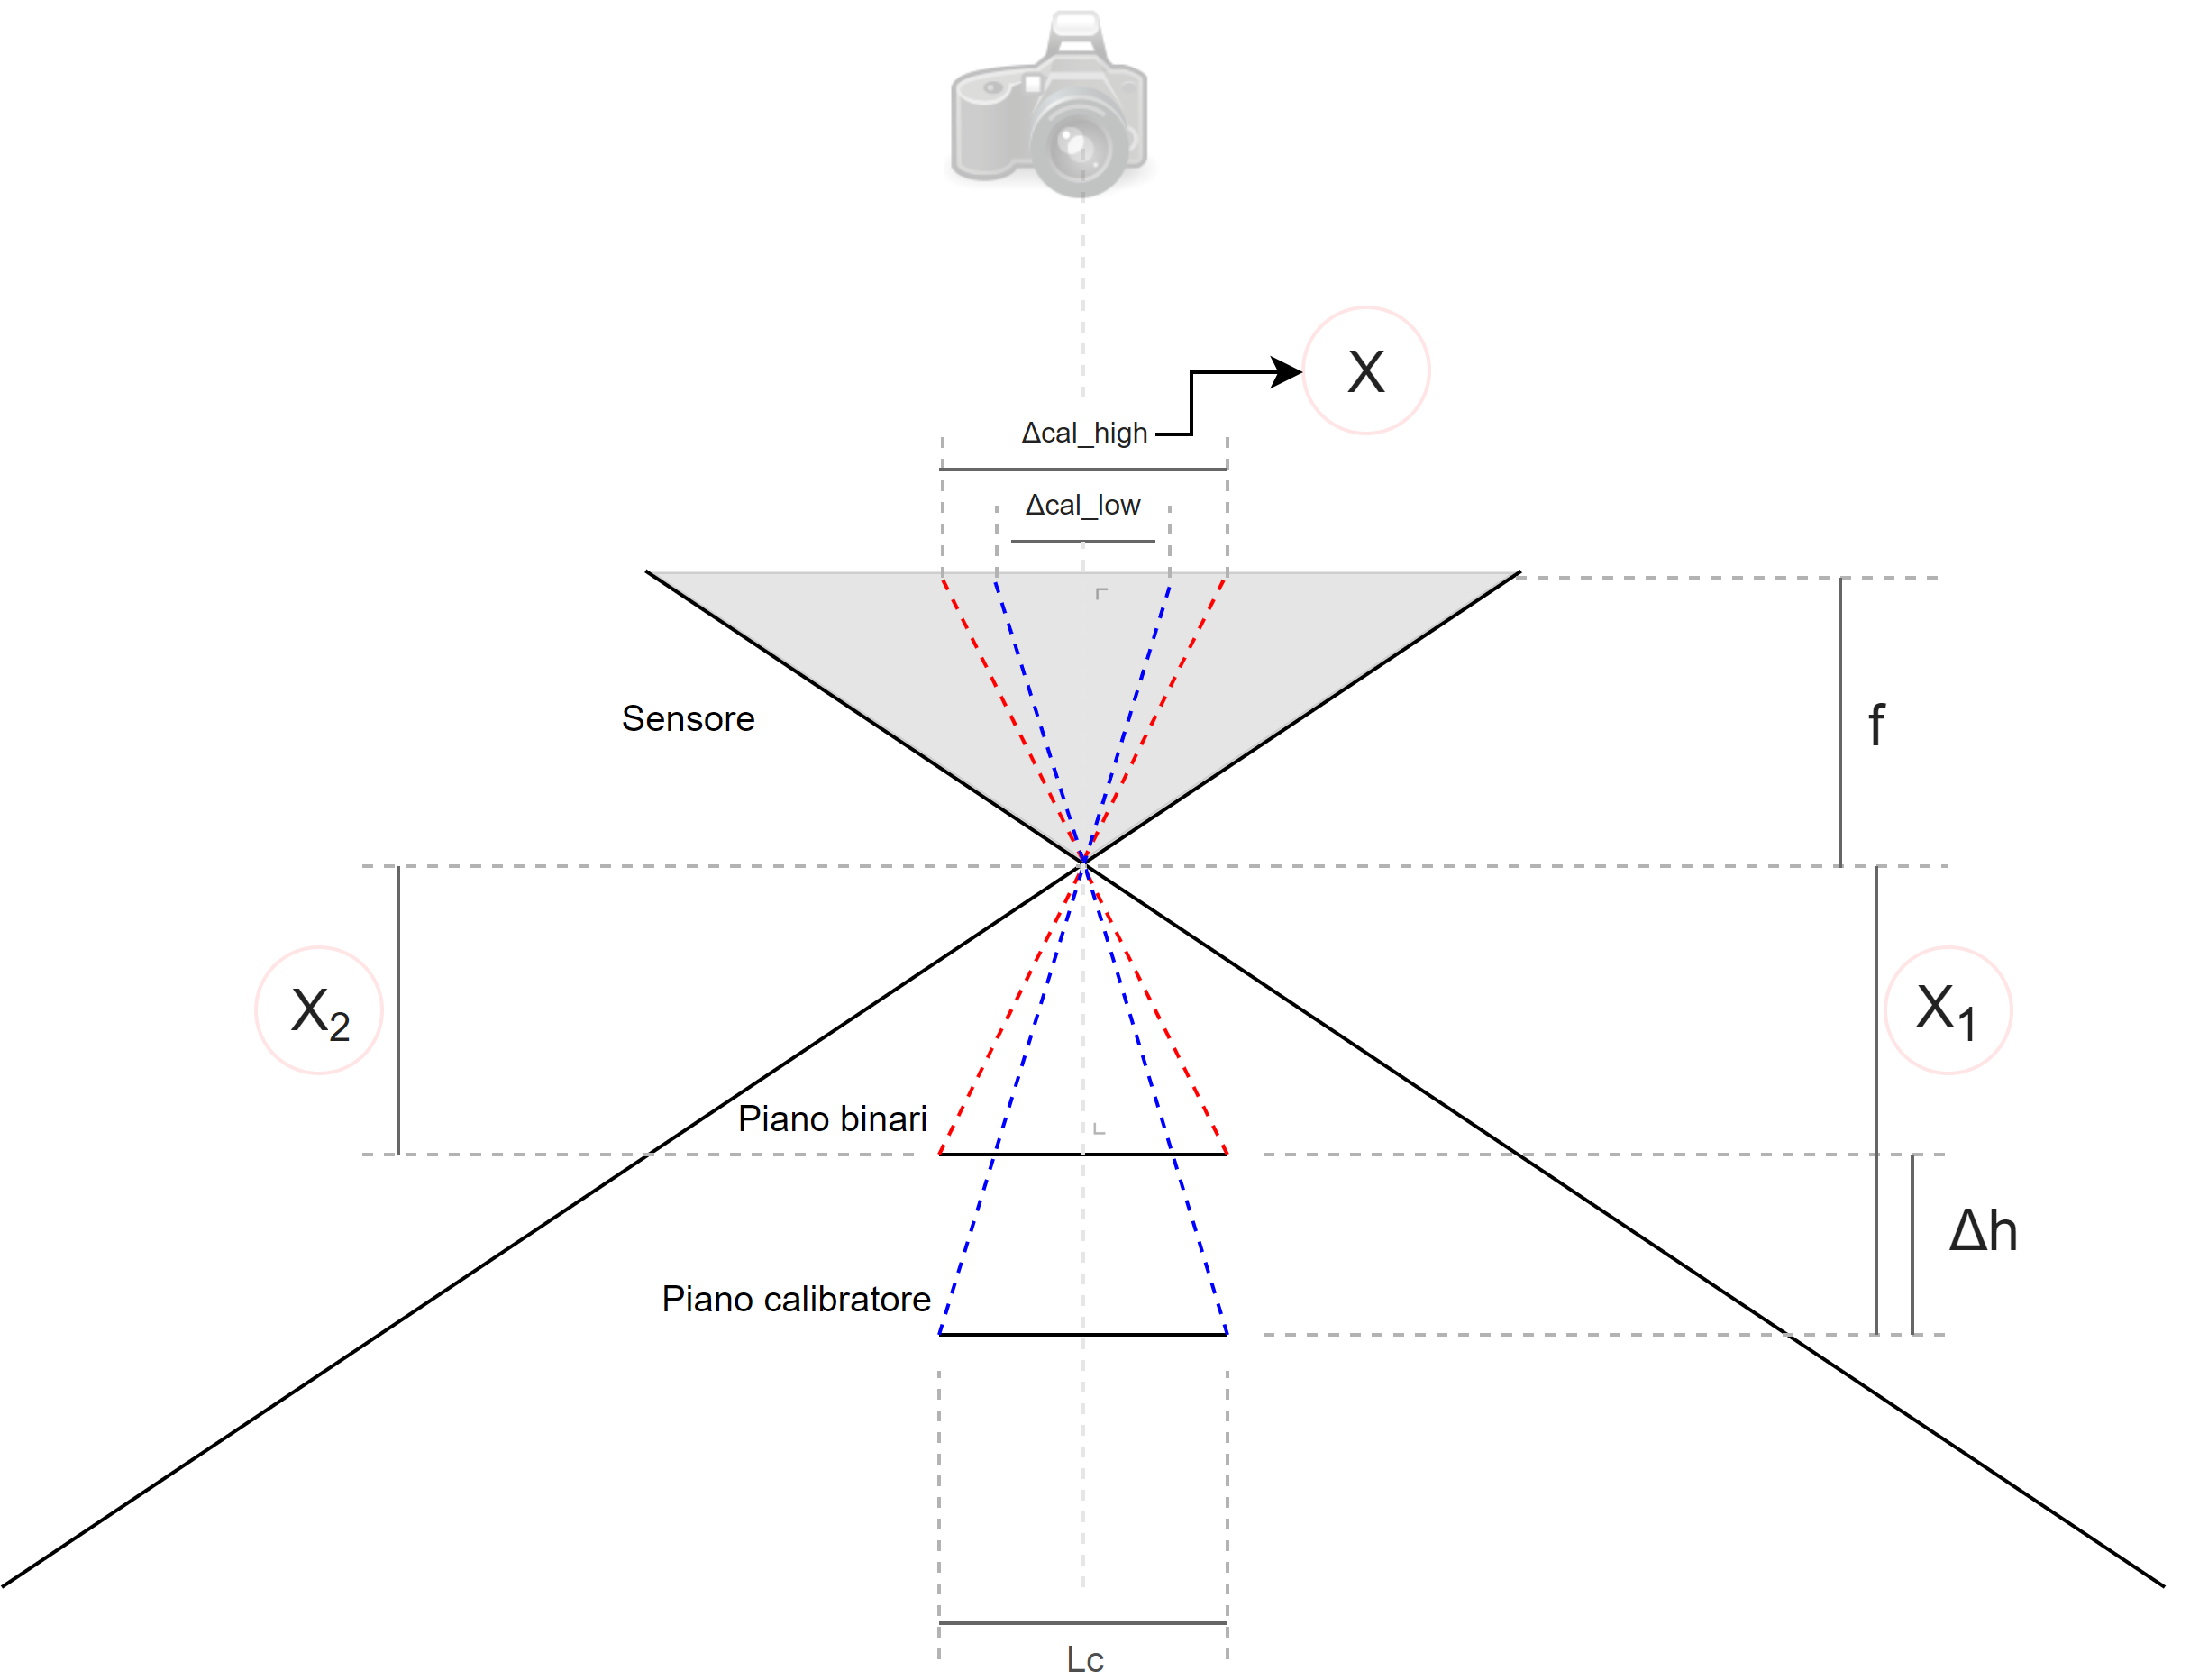
\includegraphics[scale=0.45]{images/ProblemaAltezza.png}
  \caption{Disegno esplicativo della focale}
\end{figure}
Spiegazione matematica di come riportare le misurazioni su piani paralleli differenti
\subsection{Calibrazione della camera}

\subsection{Concatenazione di più fotografie}

\subsection{Controllo online della ripresa video}

\section{Considerazioni finali}
cosa mi è piaciuto in particolare del progetto, soddisfazione etc.

\bibliographystyle{unsrt}\nocite{*}
\bibliography{bibliografia}
\end{document}
